%%%%%%%%%%%%%%%%%%% %%%%%%%%%%%%%%%%%%%%%%
% NIWeek 2014 Poster by T. Reveyrand
% www.microwave.fr
% http://www.microwave.fr/LaTeX.html
% ---------------------------------------
% 
% Original template created by:
% Brian Amberg (baposter@brian-amberg.de)
%
% This template has been downloaded from:
% http://www.LaTeXTemplates.com
%
% License:
% CC BY-NC-SA 3.0 (http://creativecommons.org/licenses/by-nc-sa/3.0/)
%
%%%%%%%%%%%%%%%%%%%%%%%%%%%%%%%%%%%%%%%%%

%----------------------------------------------------------------------------------------
%	PACKAGES AND OTHER DOCUMENT CONFIGURATIONS
%----------------------------------------------------------------------------------------

\documentclass[a0paper,portrait]{baposter}

\usepackage[font=small,labelfont=bf]{caption} % Required for specifying captions to tables and figures
\usepackage{booktabs} % Horizontal rules in tables
\usepackage{relsize} % Used for making text smaller in some places

\usepackage{amsmath,amsfonts,amssymb,amsthm, stmaryrd} % Math packages
\usepackage{eqparbox}

\usepackage{textcomp}
\usepackage{color}
\usepackage{colortbl}
\usepackage{multirow}
\usepackage{amsmath}
\DeclareMathOperator*{\argmax}{arg\,max}

\graphicspath{{figures/}} % Directory in which figures are stored

 \definecolor{bordercol}{RGB}{40,40,40} % Border color of content boxes
 \definecolor{headercol1}{RGB}{186,215,230} % Background color for the header in the content boxes (left side)
 \definecolor{headercol2}{RGB}{120,120,120} % Background color for the header in the content boxes (right side)
 \definecolor{headerfontcol}{RGB}{0,0,0} % Text color for the header text in the content boxes
 \definecolor{boxcolor}{RGB}{210,235,250} % Background color for the content in the content boxes
% \definecolor{boxcolor}{RGB}{255,255,255}
 
 \usepackage{algorithm}
\usepackage[noend]{algpseudocode} 

\usepackage[all,pdftex]{xy}
% For faster compilation. Entries must be wrapped in curly braces!
\CompileMatrices 
\xyoption{v2}
\xyoption{curve}
\xyoption{2cell}
\SelectTips{cm}{}  % Tips (of arrows) are in accordance with Computer Modern
\UseAllTwocells
%\SilentMatrices
\def\labelstyle{\textstyle}
\def\twocellstyle{\textstyle}

\newcommand{\bu}{\mathbf{u}}
\newcommand{\bv}{\mathbf{v}}

% define some signal names as abbreviations
\newcommand{\throttle}{\mathit{throttle}}
\newcommand{\brake}{\mathit{brake}}
\newcommand{\speed}{\mathit{speed}}
\newcommand{\rpm}{\mathit{rpm}}
\newcommand{\gear}{\mathit{gear}}
\newcommand{\AF}{\mathit{AF}}
\newcommand{\AFref}{\mathit{AF}_\text{ref}}

\newcommand{\DiaOp}[1]{\Diamond_{#1}}
\newcommand{\BoxOp}[1]{\square_{#1}}

\newcommand{\yes}{20*}
\newcommand{\no}{0*}

\newcommand{\Falsify}{\mathsf{Falsify}}
\newcommand{\STL}{\textbf{STL}}
\newcommand{\Rpos}{\R_{>0}}
\newcommand{\R}{{\mathbb{R}}}
\newcommand{\N}{{\mathbb{N}}}


\DeclareMathOperator*{\argmin}{arg\,min}

\newcommand{\sem}[1]{\llbracket #1 \rrbracket} 

\begin{document}

\background{ % Set the background to an image (background.pdf)
\begin{tikzpicture}[remember picture,overlay]
\draw (current page.north west)+(-2em,2em) node[anchor=north west]
{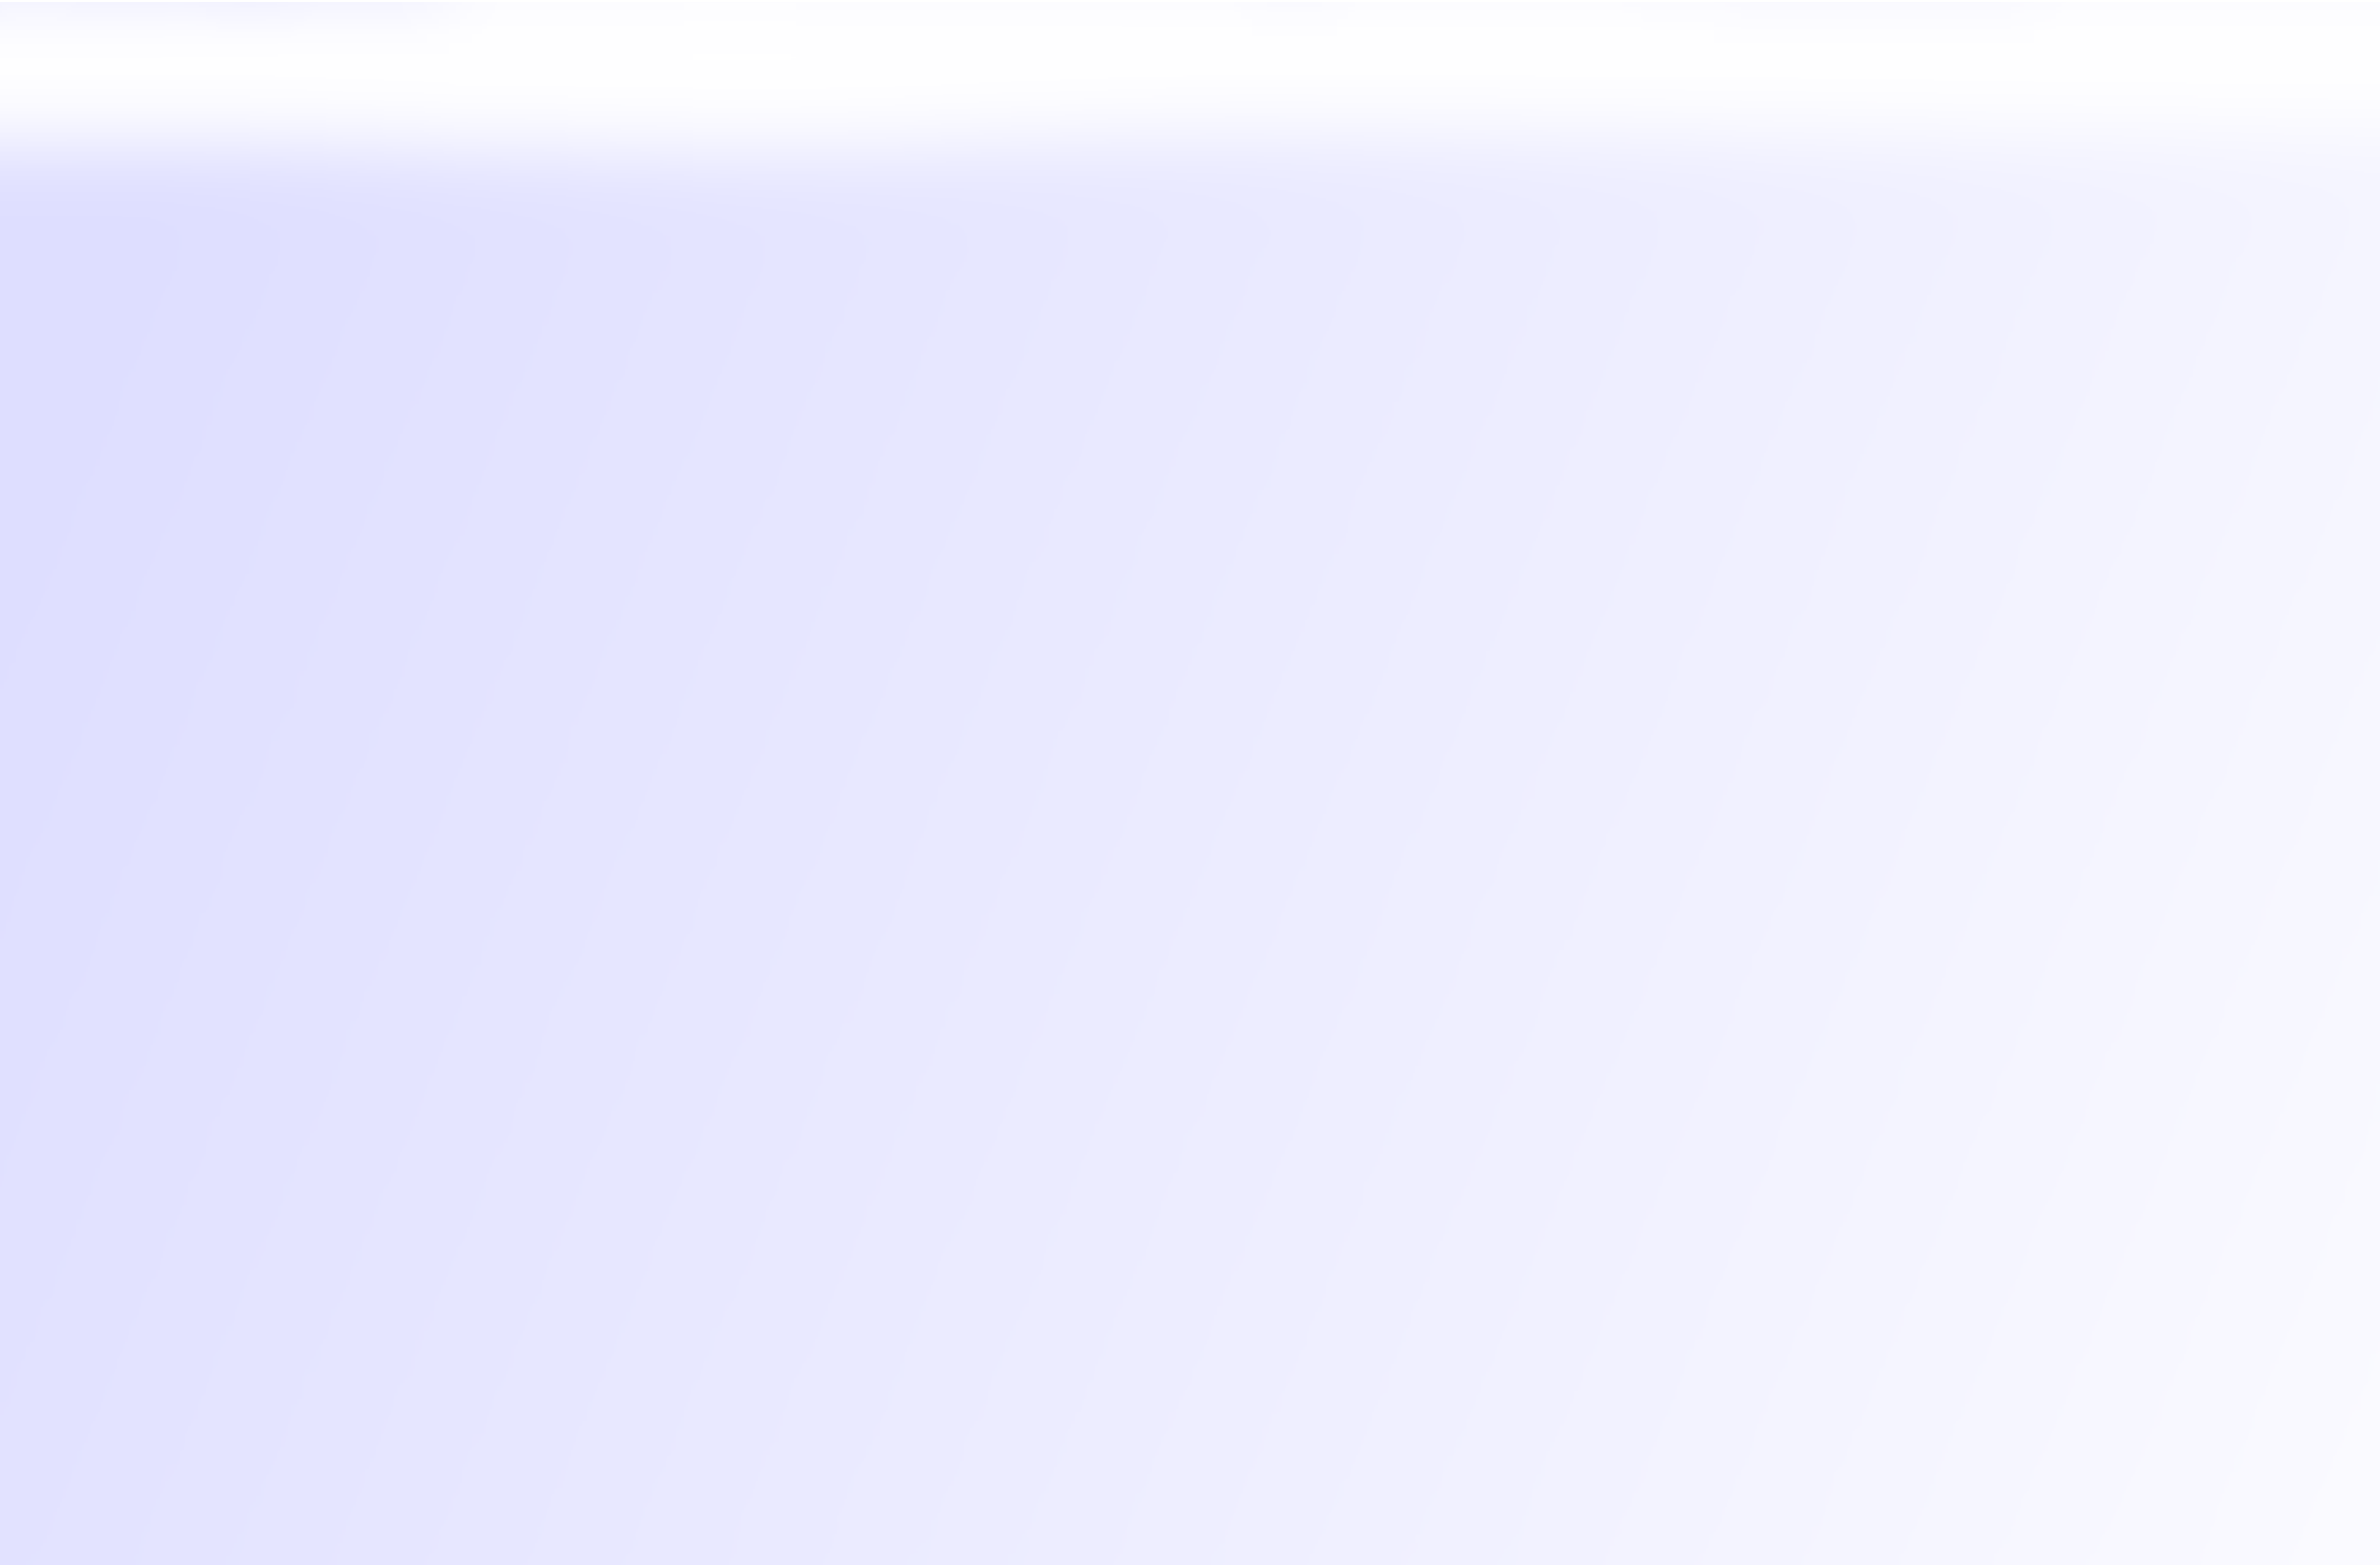
\includegraphics[height=1.1\textheight]{background}};
\end{tikzpicture}
}

\begin{poster}{
grid=false,
borderColor=bordercol, % Border color of content boxes
headerColorOne=headercol1, % Background color for the header in the content boxes (left side)
headerColorTwo=headercol2, % Background color for the header in the content boxes (right side)
headerFontColor=headerfontcol, % Text color for the header text in the content boxes
boxColorOne=boxcolor, % Background color for the content in the content boxes
headershape=roundedright, % Specify the rounded corner in the content box headers
headerfont=\Large\sf\bf, % Font modifiers for the text in the content box headers
textborder=rectangle,
background=user,
headerborder=open, % Change to closed for a line under the content box headers
boxshade=plain
}
{
\includegraphics[scale=0.2]{erato.png}}
%
%----------------------------------------------------------------------------------------
%	TITLE AND AUTHOR NAME
%----------------------------------------------------------------------------------------
%
{\huge    {Two-Layered Falsification of Hybrid Systems Guided by \\Monte Carlo Tree Search} } % Poster title
{\vspace{0.3em} \smaller Zhenya Zhang$^{1,2}$, Gidon Ernst$^1$, Sean Sedwards$^3$,  Paolo Arcaini$^1$, Ichiro Hasuo$^{1,2}$  \\  % Author names
  
\smaller $^1$\it {National Institute of Informatics, Tokyo, Japan}\\ $^2$\it{The Graduate University for Advanced Studies, Hayama, Japan}  \\ $^3$\it{University of Waterloo, Waterloo, Canada} } % Author email addresses
%{\includegraphics[scale=0.45]{NI.jpg}} % University/lab logo

%----------------------------------------------------------------------------------------
%	INTRODUCTION
%----------------------------------------------------------------------------------------
\headerbox{Problem}{name=introduction,column=0,row=0, span=3}{

\begin{itemize}



\item Falsification problem is defined as follows:
%In formal verification one aims to give a mathematical proof for a system's correctness. This is much harder for hybrid systems than for computer software/hardware, %. One reason is theoretical:
% where the presence of continuous dynamics makes many problems more complex or even undecidable (e.g.\ reachability in hybrid automata). 
% \begin{minipage}{0.65\textwidth}
%    \underline{\bfseries The falsification problem}
\vspace{-0.5em} 
    \begin{itemize}
    \item{\textbf{Given:}} 
      a \emph{model} $\mathcal{M}$ (that takes an input signal $\bu$
      and  yields  an output signal $\mathcal{M}(\bu)$), and
      a \emph{specification} $\varphi$ (a temporal formula) 
      \vspace{-0.3em}
    \item{\textbf{Answer:}} 
      \emph{error input}, that is, an input signal $\bu$ such
      that the corresponding output $\mathcal{M}(\bu)$ violates $\varphi$ 
    \end{itemize}
 % \end{minipage}



\vspace{-0.6em}
\item Challenges:
\vspace{-1.5em} 

\begin{itemize}
	\vspace{-0.3em} 
\item Black/Grey box model, e.g., model in Simulink, etc.
\hspace{6em}
\begin{minipage}{0.4\textwidth}
\centering
  \begin{math} 
   \xymatrix@1@+2.5em{
   {}
     \ar[r]^-{\bu}
   &
   {  \quad\xybox{ *++++[F]{\mathcal{M}} }}
     \ar[r]^-{\mathcal{M}(\bu)}_-{\not\models\varphi \; ?}
   &
   {}
   }
  \end{math}
 \end{minipage}
\vspace{-1.5em} 
\item Continuous (infinite) input space
\end{itemize}
\end{itemize}

}


%----------------------------------------------------------------------------------------
%	CALIBRATION
%----------------------------------------------------------------------------------------
\headerbox{Preliminary}{name=relwork, column=0, below=introduction}{

Robust semantics of temporal formulas
\vspace{-0.6em}
\begin{itemize}
\item Boolean satisfaction:   $\bv\models\varphi$ or $\bv\not\models\varphi$ 
\vspace{-0.6em}
\item Quantitative robustness:\\ $\sem{\bv,\varphi}\in\R\cup\{\infty,-\infty\}$ %$\sem{\mathbf{v}_2,\varphi} = -10$
\end{itemize}
\vspace{-0.6em}

Optimization-based technique: 
\vspace{-0.6em}
\begin{itemize}
\item Goal: $\min \sem{\bv,\varphi}$
\vspace{-0.6em}
\item ``Hill-Climbing'' algorithms: CMA-ES, Nelder-Mead,  Simulated Annealing, etc. %$\sem{\mathcal{M}(\bu^{(i+1)}),\varphi} > \sem{\mathcal{M}(\bu^{(i)}),\varphi}$    
\end{itemize}



}




\headerbox{Optimization-based method}{name=optsolver, column=0, below=relwork}{

%\quad  $\bullet \quad\Box~(\speed < 120)$


 \centering 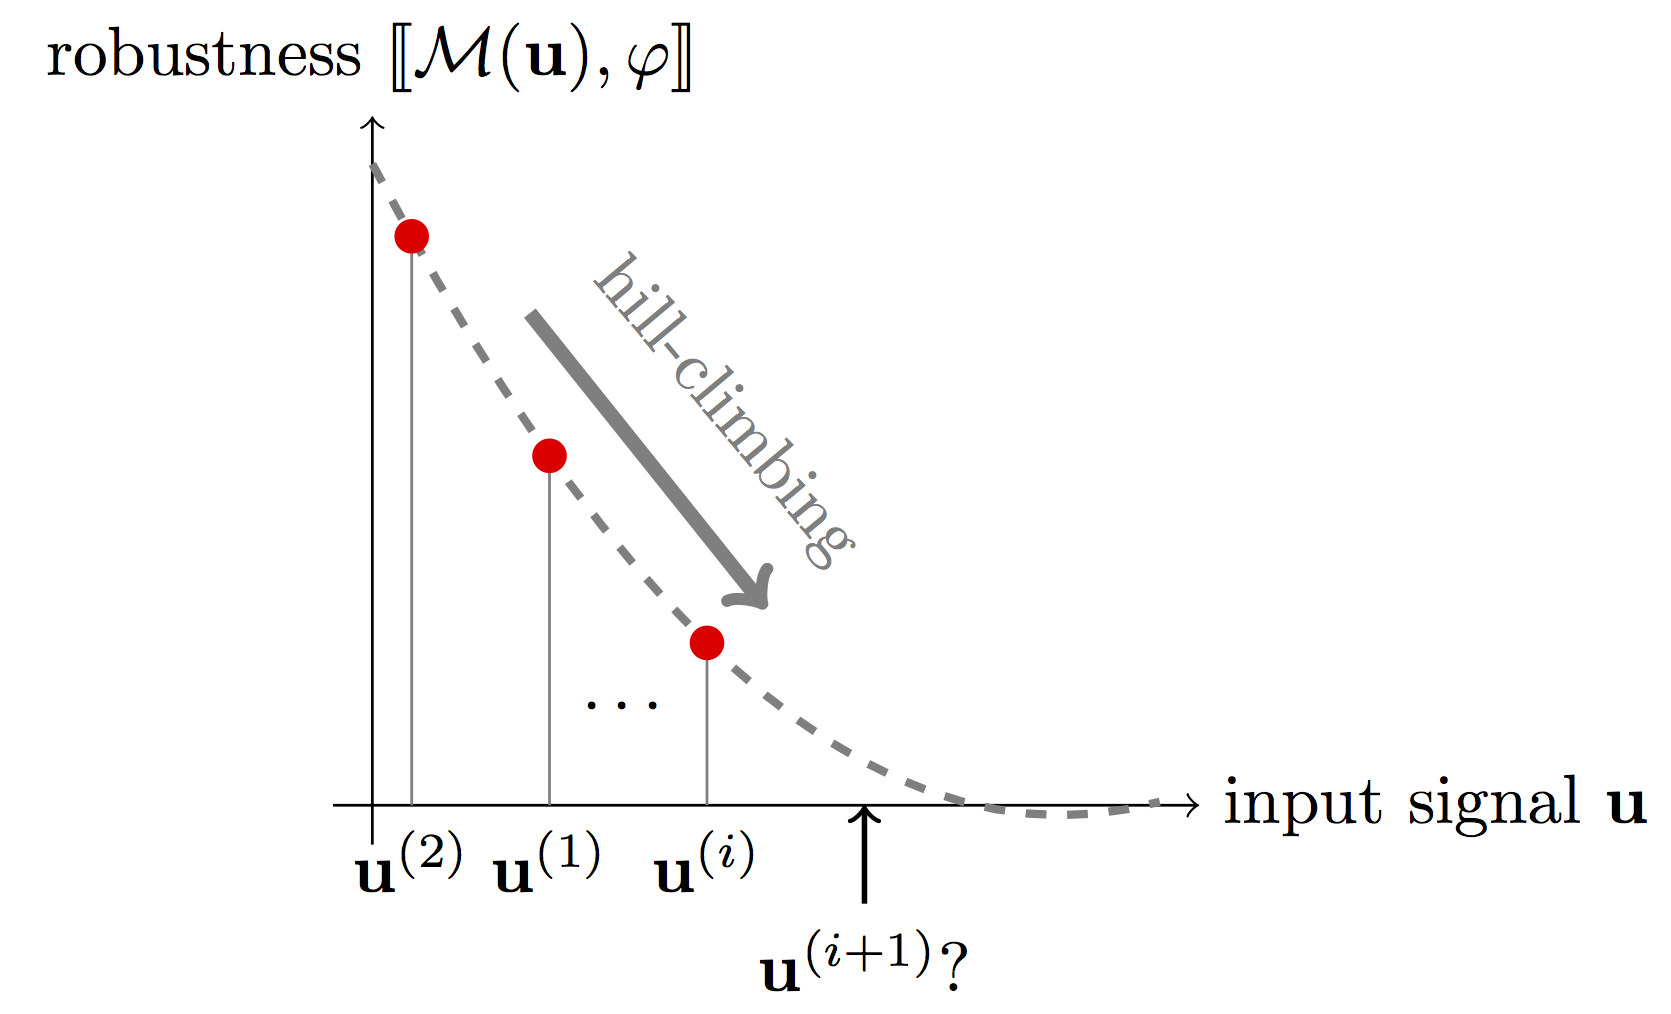
\includegraphics[scale=.08]{figures/figHillClimbing.png}
  \vspace{-0.2em}
 
  \raggedright ``Hill-Climbing'' algorithm:
    \vspace{-0.6em}
  \begin{itemize}
\item In the $i$-th sampling one tries an input signal $\bu^{(i)}$. The corresponding output signal $\bv^{(i)}=\mathcal{M}(\bu^{(i)})$ is shown below it.
\vspace{-0.6em}
\item Optimization algorithm decides a new input signal 
$\bu^{(i+1)}=(u_{1}^{(i+1)},\dotsc,u_{K}^{(i+1)})$. %It is in the choice
and $\bu^{(i+1)}$ makes the robustness smaller. 
\end{itemize}

  
}

\headerbox{Monte Carlo Tree Search}{name=overview, column=0, below=optsolver}{
Monte Carlo Tree Search (MCTS) is a heuristic search algorithm that focuses more on those promising branches rather than the whole tree. A general MCTS usually contains 4 steps:

\centering 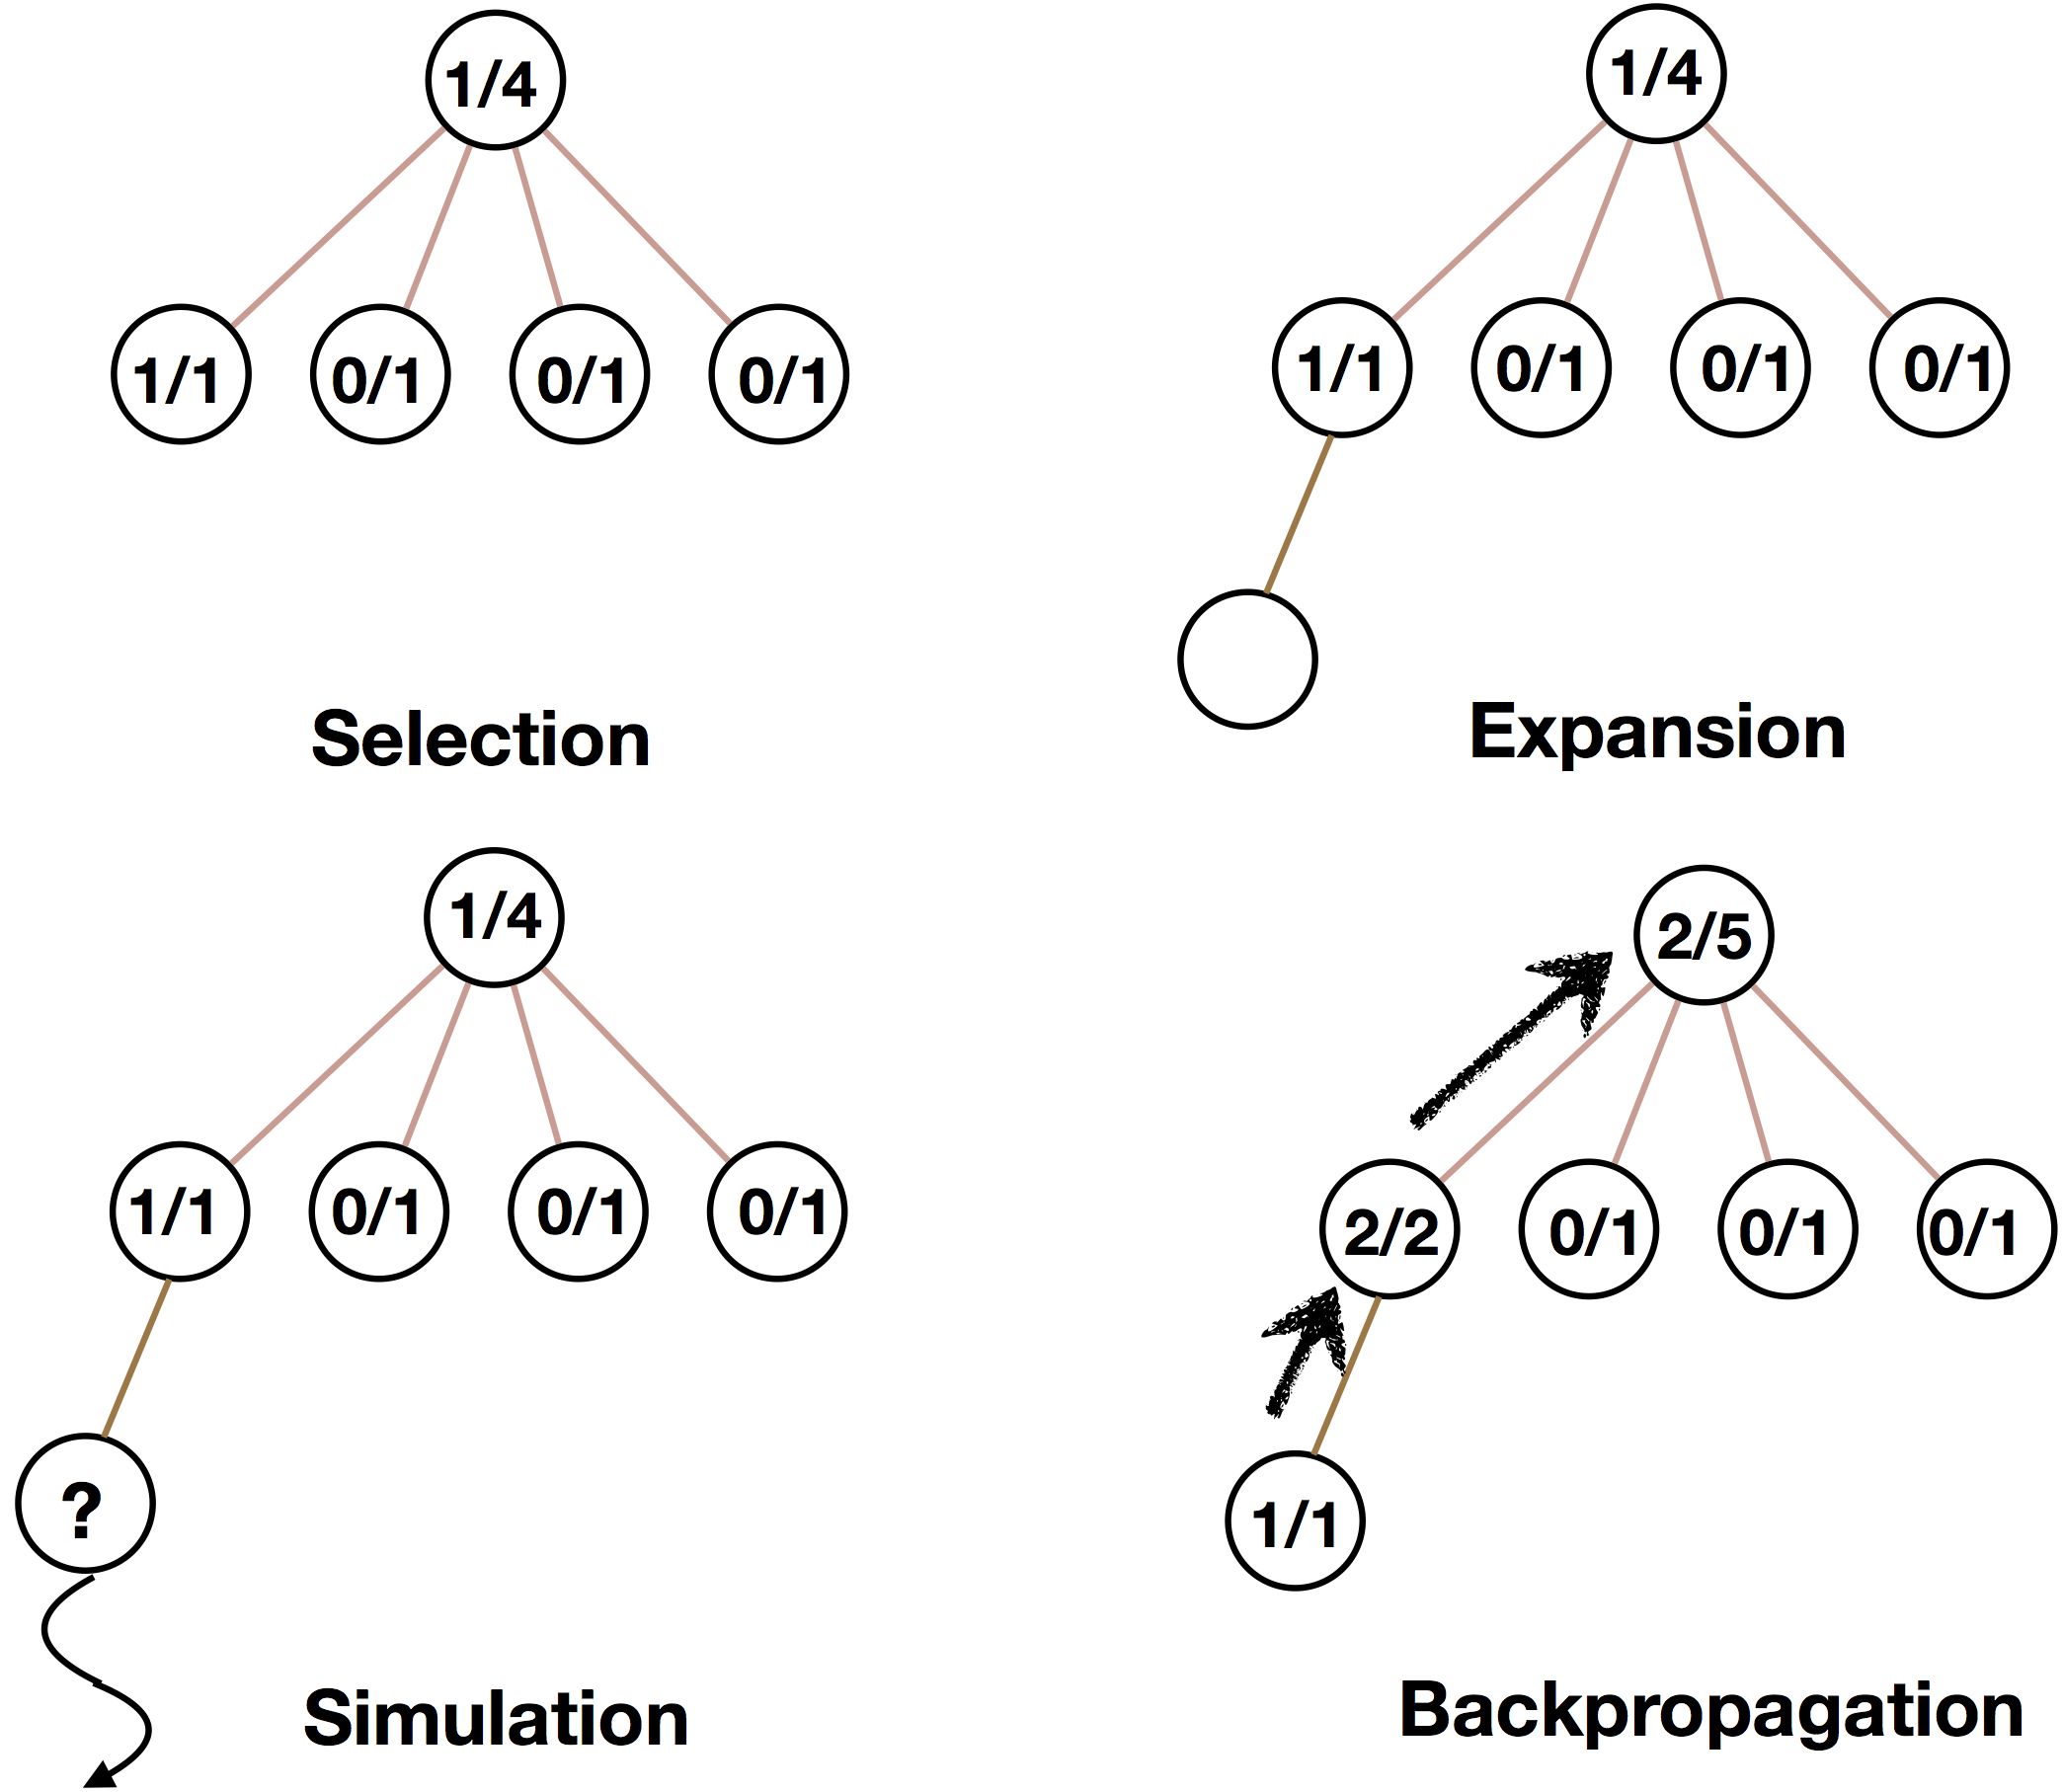
\includegraphics[scale=.083]{figures/mctsfig.png}

\begin{enumerate}
\item Selection: select one ``promising'' child according to UCB1 algorithm.
\vspace{-0.6em}
\item Expansion: create a new child.
\vspace{-0.6em}
\item Simulation: randomly select a sequence of children until the game is decided, and record the result.
\vspace{-0.6em}
\item Backpropagation: update the winning and visiting times of the nodes in the path.
\end{enumerate}

}


%----------------------------------------------------------------------------------------
%	OTHER INSTRUMENTATION
%----------------------------------------------------------------------------------------
\headerbox{Algorithm overview}{name=algorithm,span=2,column=1,row=1, below=introduction}{ % To reduce this block to 1 column width, remove 'span=2'

\centering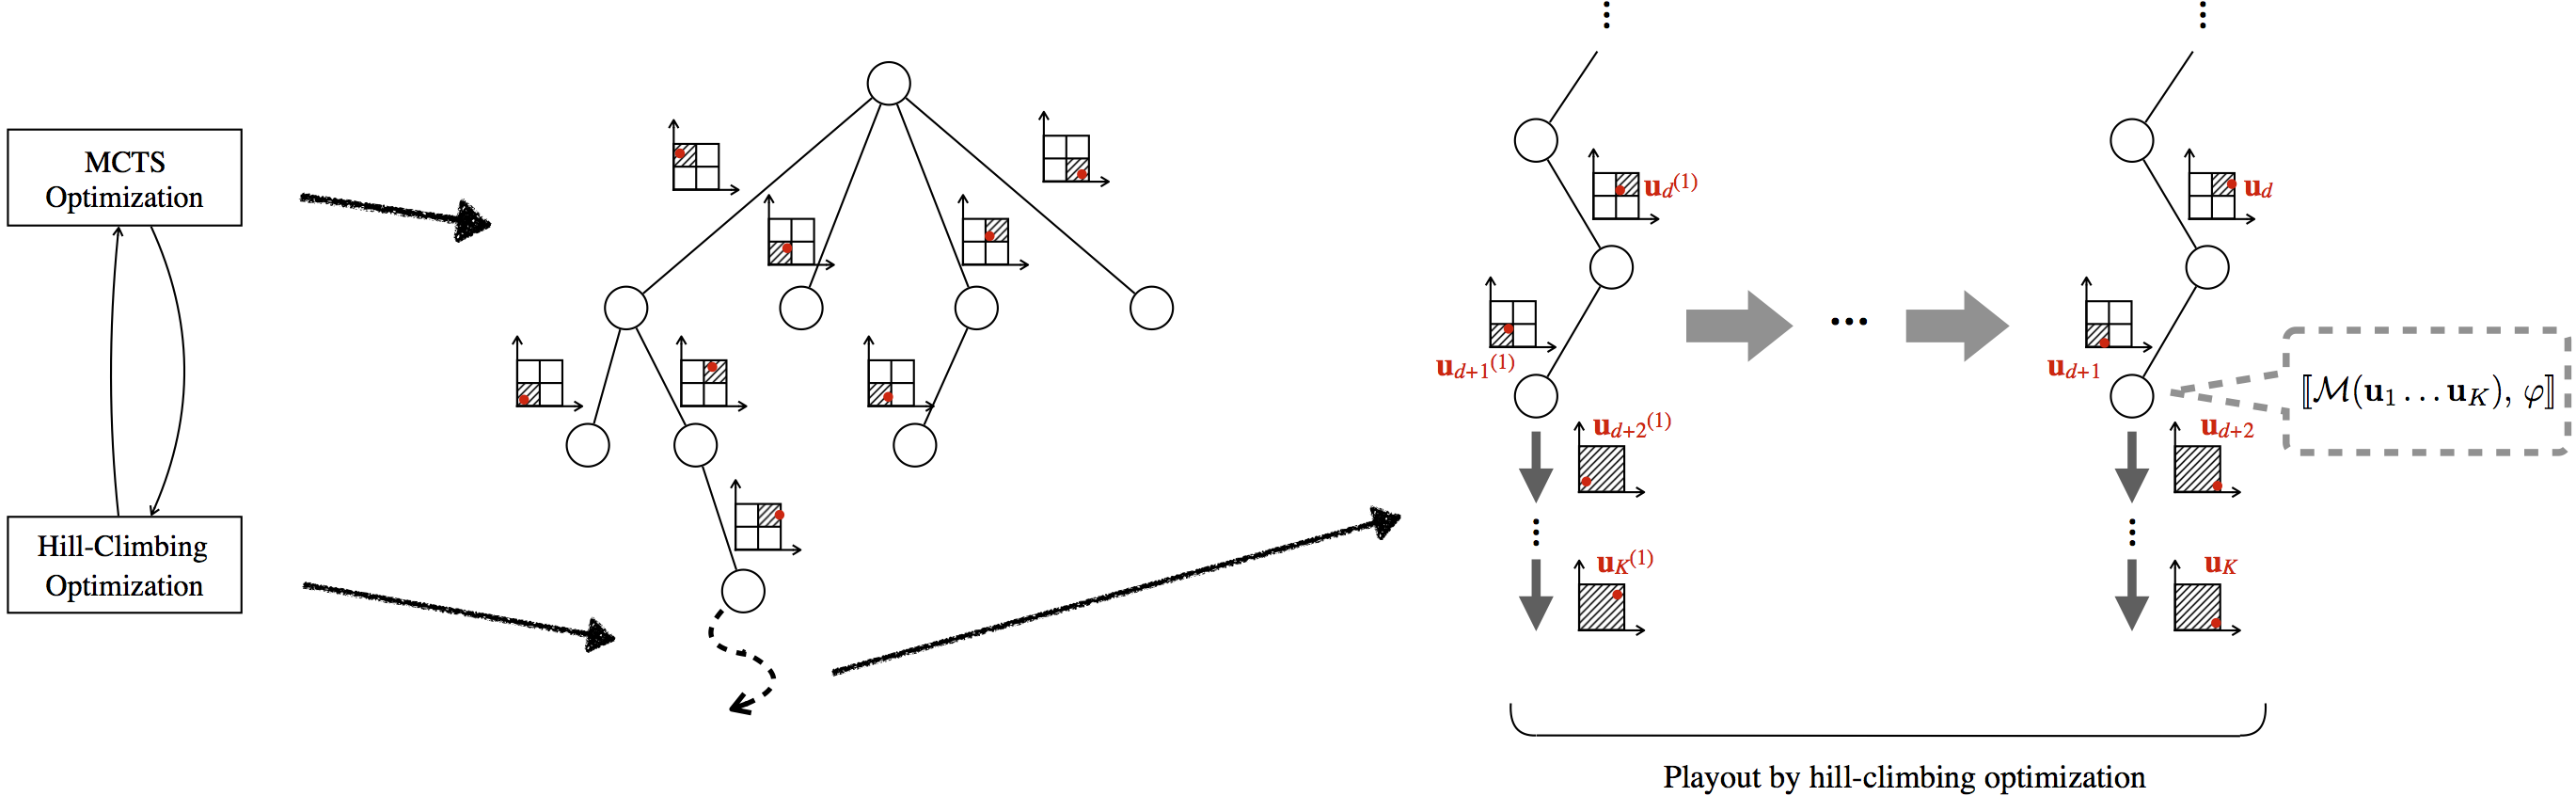
\includegraphics[scale=.14]{figures/algorithm.png}

\raggedright
Basic algorithm:
\begin{itemize}
\vspace{-0.6em}
\item Time-staging. Divide the time bound into $K$ intervals to find a sequence $\bu_{1},\dotsc,\bu_{K}$.


\vspace{-0.6em}
\item Node expansion. Use a \emph{partitioning} of the input space $I_{1}\times\cdots\times I_{M}$ as the children set $A$.
\vspace{-0.6em}

\item Child selection. Define that $reward = 1-\frac{R(wa)}{\max_{w'\in\mathcal{T}}R(w')}$, and apply UCB1 algorithm $\argmax_{a\in A} \left(reward + c\sqrt{\frac{2\ln N(w)}{N(wa)}}\right)$ to select the best child.
\vspace{-0.6em}

\item Simulation. Apply optimization solvers in the selected sub-region sequence with time budget.

\vspace{-0.6em}


\item Backpropagation. Update the reward of parent if the newly computed reward is better.

\vspace{-0.6em}

\item Postprocessing. Apply optimization algorithm again if no solution is returned.

\end{itemize}
\vspace{-0.6em}
Variation:
\begin{itemize}
\vspace{-0.6em}
\item Progressive widening. Unlike the basic algorithm, the children of higher layer are possible to be expanded earlier than the children on the second layer. 

\end{itemize}

}


%----------------------------------------------------------------------------------------
%	MIXER vs. SAMPLERS
%----------------------------------------------------------------------------------------
\headerbox{Experimental evaluation}{name=autotrans, span=2, column=1, row=1, below=algorithm}{

%\begin{small}\centering
\newcommand{\tbcolor}{\cellcolor{white!25}}
\scalebox{0.62}{
%\setlength\tabcolsep{3.5pt}

\begin{tabular}{llrrrrrrrrrrrrrrrrrrrr}
\toprule
    &
    %& \multicolumn{3}{l}{~Parameters}
    & \multicolumn{10}{l}{~AT model}
    & \multicolumn{4}{l}{~AFC model}
    &\multicolumn{2}{l}{~FFR model}
    \\
%\cmidrule(lr){3-5}
\cmidrule(lr){3-12}
\cmidrule(l){13-16}
\cmidrule(l){17-18}
    &
    %&
    %&
    %&
    & \multicolumn{2}{c}{S1}
    & \multicolumn{2}{c}{S2}
    & \multicolumn{2}{c}{S3}
    & \multicolumn{2}{c}{S4}
    & \multicolumn{2}{c}{S5}
    & \multicolumn{2}{c}{Sbasic}
    & \multicolumn{2}{c}{Sstable}
    & \multicolumn{2}{c}{Strap}
    \\
   \multicolumn{2}{c}{Algorithm}
    %& M\_b & $\text{TO}_\text{po}$
    %& \multicolumn{1}{c}{$c$}
    & succ. & time
    & succ. & time
    & succ. & time
    & succ. & time
    & succ. & time
    & succ. & time
    & succ. & time
    & succ. & time
    \\
\cmidrule(r){1-2}
%\cmidrule(lr){3-5}
\cmidrule(lr){3-4}
\cmidrule(lr){5-6}
\cmidrule(lr){7-8}
\cmidrule(lr){9-10}
\cmidrule(lr){11-12}
\cmidrule(lr){13-14}
\cmidrule(lr){15-16}
\cmidrule(l){17-18}

 \multicolumn{2}{c}{Random}  &   10/10 &  108.9 & 10/10 &   289.1 &      1/10 & 301.1 &  0/10 &  - &  0/10 &  -  &  6/10  & 278.7   &    \tbcolor  10/10 & \tbcolor 242.6  &4/10 & 409.3  \\\midrule
\multirow{3}{*}{\rotatebox{90}{\begin{footnotesize}CMA-ES\end{footnotesize}}}
& Breach &    10/10 &  21.9 & 6/10 &   30.3 & \textbf{10/10} & \textbf{193.9} &   4/10 & 208.8 &  3/10 &  75.5  & \tbcolor \textbf{10/10}   &  \tbcolor\textbf{111.7}   &      3/10 &  256.3&\tbcolor\textbf{10/10} &\tbcolor\textbf{119.8} \\
& Basic   & 10/10 &  15.8 & 10/10 & 108.5 & 10/10 & 697.1  &  7/10 & 786.8 &  9/10 & 384.4   & 10/10& 182.0   &7/10&336.9& 10/10 &338.0 \\
& P.W.   &  \textbf{10/10} &  \textbf{10.8} & \tbcolor\textbf{10/10} &\tbcolor \textbf{65.7} &  10/10 & 728.6 &  \textbf{7/10} & \textbf{767.8} &  \textbf{10/10} & \textbf{648.1}&  10/10 & 177.1 &\textbf{8/10}&\textbf{272.9}&10/10 &473.9\\
\midrule
\multirow{3}{*}{\rotatebox{90}{GNM}}
& Breach &     \tbcolor\textbf{10/10} &  \tbcolor\textbf{5.4} & \textbf{10/10} & \textbf{151.4} &  0/10 &     - &  0/10 &     - &  0/10 &     -
&  \textbf{10/10}& \textbf{171.4}      & 0/10&- & 0/10 & - \\
& Basic   & 10/10 &  12.4 & 10/10 & 162.3 &\tbcolor\textbf{10/10} &\tbcolor\textbf{185.6}  &  7/10 & 261.9 &  7/10 & 163.7&    10/10&  227.1     & 2/10&378.5& \textbf{10/10}&\textbf{162.2}\\
& P.W.   &  10/10 & 60.8 &  9/10 & 110.7 &  8/10 & 211.2  & \tbcolor \textbf{8/10} & \tbcolor\textbf{313.0} & \tbcolor\textbf{10/10} &\tbcolor\textbf{178.7} &  10/10& 252.0   &\textbf{6/10}&\textbf{153.2}& 6/10 &197.4\\
\midrule
\multirow{3}{*}{\rotatebox{90}{SA}}
& Breach &     \textbf{10/10} & \textbf{160.1} &  0/10 &     - &  3/10 & 383.7 &  0/10 &     - &  3/10 &  80.4 &   0/10&  -    &6/10&307.0& 3/10 & 92.8\\
& Basic   &  10/10 & 264.8 &  9/10 & 236.1 & \textbf{8/10} & \textbf{385.6}  &  \textbf{8/10} & \textbf{505.3} &  7/10 & 341.2 &    5/10&391.3  &\textbf{8/10}& \textbf{273.8}& \textbf{10/10} &\textbf{273.2} \\
& P.W.   &  10/10 & 208.7 & \textbf{10/10} & \textbf{377.6} &  8/10 & 666.0  &  7/10 & 795.4 & \textbf{10/10} & \textbf{624.2}&   \textbf{8/10}   &  \textbf{665.7}     &6/10&293.7&10/10 &390.9\\
\bottomrule
\end{tabular}

}


\begin{minipage}[h]{0.53\textwidth}
%\raggedright
\begin{small}
\textbf{S1} $\Box_{[0,30]}~(\speed < 120)$

\textbf{S2} $\Box_{[0,30]}~(\gear = 3 \to \speed \ge 20)$

\textbf{S3} $\Diamond_{[10,30]}~(\speed \le 53 \lor \speed \ge 57)$

\textbf{S4} $\Box_{[0,29]}~(\speed < 100) \lor \Box_{[29,30]}(\speed > 65)$

\textbf{S5} $\Box_{[0,30]}(\rpm < 4770 \lor \Box_{[0,1]}(\rpm > 600))$ 

\textbf{Sbasic} $\Box_{[11,30]}(\neg(|\AF-\AFref|>0.05*14.7))$


\textbf{Sstable} $\neg(\DiaOp{[6,26]}{\BoxOp{[0,4]}{(\AF - \AFref > 0.01 * 14.7))}}$

\textbf{Strap} $\neg\DiaOp{[0,5]}(x,y\in[3.9,4.1]\wedge\dot{x},\dot{y}\in [-1,1])$
\end{small}

\end{minipage}
\begin{minipage}[h]{0.45\textwidth}
\begin{small}
%\centering
\raggedright Model:
\begin{itemize}
\vspace{-0.6em}
\item AT: Automatic Transmission
\vspace{-0.6em}
\item AFC: Abstract Fuel Control
\vspace{-0.6em}
\item FFR: Free Floating Robot
\vspace{-0.6em}
\end{itemize}

Algorithm:
\begin{itemize}
\vspace{-0.6em}
\item Breach: optimization
\vspace{-0.6em}
\item Basic: MCTS + Hill-Climbing
\vspace{-0.6em}
\item P.W.: MCTS + Hill-Climbing + progressive widening
\vspace{-0.6em}
\end{itemize}

\end{small}

\end{minipage}




%\end{small}
}


%----------------------------------------------------------------------------------------
%	MEASUREMENT SETUP
%----------------------------------------------------------------------------------------



%----------------------------------------------------------------------------------------
%	CONCLUSION
%----------------------------------------------------------------------------------------
\headerbox{Conclusion \& Future work }{name=conclusion,column=1,below=autotrans,span=2}{
In this work we have presented a two-layered optimization framework for hybrid system falsification. It combines Monte Carlo tree search—a widely used stochastic search method that effectively balances exploration and exploitation—and hill-climbing optimization—a local search method whose use in hybrid system falsification is established in the community. Our experiments demonstrate its promising performance.

\vspace{0.55em}
Two directions for future work:
\begin{itemize}
\vspace{-0.7em}
\item Compute a quantitative coverage metric from the result of our MCTS algorithm.
\vspace{-0.7em}
\item Explore variations of robust semantics
to mitigate discrete propositions.
\end{itemize}


}


%----------------------------------------------------------------------------------------
%	REFERENCES
%----------------------------------------------------------------------------------------

%\headerbox{References}{name=references,column=2,below=application}{

%\smaller % Reduce the font size in this block
%\renewcommand{\section}[2]{\vskip 0.05em} % Get rid of the default "References" section title
%\nocite{*} % Insert publications even if they are not cited in the poster

%\bibliographystyle{unsrt}
%\bibliographystyle{IEEEtran}
%\bibliography{biblio} % Use biblio.bib as the bibliography file
%}


%----------------------------------------------------------------------------------------
%	ACKNOWLEDGEMENTS
%----------------------------------------------------------------------------------------

\headerbox{Acknowledgements}{name=acknowledgements,column=0,below=conclusion, above=bottom,span=3}{

This work is supported by ERATO HASUO Metamathematics for Systems Design Project
(No. JPMJER1603), Japan Science and Technology Agency.
} 


\end{poster}

\end{document}